\chapter{Gaussian Probabilistic Latent Semantic Analysis}
\label{chp:gplsa}

\hspace{0.1in}
\section{Problem Settings}

Suppose that we have a target task $\mathcal{D}$ where we wish to solve the rating prediction problem. Taking the regular recommendation system for illustration, $\mathcal{D}$ is associated with $m_{d}$ users and $n_{d}$ items denoted by $\Us^{d}$ and $\Is^{d}$ respectively. In this task, we observe a sparse matrix $\X^{(d)}\in \mathbb{R}^{m_d\times n_{d}}$ with entries $x^d_{ui}$. Let $\R^{(d)}=\{(u,i,r):r=x^d_{ui},\mbox{where } x^d_{ui}\ne 0\}$ denote the set of observed links in the system. For the rating recommendation system, $r$ can either take numerical values, for example $[1,5]$, or binary values $\{0, 1\}$. We aim to transfer knowledge from other $N$ source domains $\mathcal{S}=\{S^t\}_{t=1}^{N}$ with each source domain $S^t$ contains $m^t_s$ users and $n^t_s$ items denoted by $\Us^{s^t}$ and $\Is^{s^t}$. Similar to the target domain, each source domain $S^t$ contain sparse matrices $\X^{(s^t)}\in \mathbb{R}^{m_{s^t}\times n_{s^t}}$ and observed links $\R^{(s^t)}=\{(u,i,r):r=x^{s^t}_{ui},\mbox{ where } x^{s^t}_{ui}\ne 0\}$.

The settings of STLCF are illustrated in Figure \ref{fig:illustration}. As shown in the figure, the first row illustrates the case where items that are in the target domain also appear in the source domains. A real-world example is the rating prediction for the movies that appear in several web sites in various forms; the second row illustrates the case where users that are in the target domain also appear in the source domains. A real-world example is the Douban recommendation system \footnote{\url{http://www.douban.com}}, which provides music, book and movie recommendation for users. We adopt a setting commonly used in transfer learning for collaborative filtering: either the items or the users that are in the target domain also appear in the source domains. In the following derivation and description of our STLCF model, for the convenience of interpretation, we focus on the case that the user set is shared by both the target domain and the source domains.
The case that the item set is shared can be easily tackled in a similar manner.

\begin{figure}
\centering
\includegraphics[width=6in]{fig/illustration.eps}
\caption{Illustration of Selective Transfer Learning with multiple sources.}
\label{fig:illustration}
\end{figure}
%$\mathcal{S}^{t}$

Under the assumption that the observation $\R^{(\{d, s^t\})}$ is obtained with $u$ and $i$ being independent, we formally define a co-occurrence model in both the target and the source domains to solve the collaborative filtering problem:
\begin{eqnarray}
\nonumber
Pr(x^{\{d, s^t\}}_{ui}=r,u,i) \!\!\!\!\!\!&=&\!\!\!\!\!\! Pr(u) Pr(i \mid u) Pr(x^{\{d, s^t\}}_{ui}=r \mid u,i) \\
\nonumber
\!\!\!\!\!\!&=&\!\!\!\!\!\! Pr(u) Pr(i) Pr(x^{\{d, s^t\}}_{ui}=r \mid u,i) \\
\nonumber
\!\!\!\!\!\!&\propto&\!\!\!\!\!\! Pr(x^{\{d, s^t\}}_{ui}=r \mid u,i)
\end{eqnarray}

In the following, based on Gaussian probabilistic latent semantic analysis (GPLSA), we first briefly present a transfer learning model for collaborative filtering - transferred Gaussian probabilistic latent semantic analysis (TGPLSA) as an example, which is designed to integrate into our later proposed framework as a base model. After that, we present our selective transfer learning for collaborative filtering (STLCF) to perform knowledge transfer by analyzing the inconsistency between the observed data in target domain and the source domains. Careful readers shall notice that other than the TGPLSA example, STLCF is compatible to use various generative models as the base model.

\hspace{0.1in}
\section{Collaborative Filtering via Gaussian Probabilistic Latent Semantic Analysis (GPLSA)}
Following ~\cite{DBLP:conf/sigir/Hofmann03}, for every user-item pair, we introduce hidden variables $Z$ with latent topics $z$, so that user $u$ and item $i$ are rendered conditionally independent. With the observations of item set $\Is$, user set $\Us$ and rating set $\R$ in the source domain, we define:
\begin{eqnarray}
\nonumber
Pr(x_{ui} = r | u, i) = \sum_{z} Pr(x_{ui} = r \mid i, z) Pr(z \mid u)
\end{eqnarray}
\vspace{-5mm}

We further investigate the use of a Gaussian model for estimating $p(x_{ui} = r | u, i)$ by introducing $\mu_{iz} \in \mathcal{R}$ for the mean and $\sigma_{iz}^2$ for the variance of the ratings. With these, we define a Gaussian mixture model for a single domain as:
\begin{eqnarray}
\nonumber
Pr(x_{ui} = r | u, i) = \sum_{z} Pr(z | u) Pr(r; \mu_{iz}, \sigma_{iz})
\end{eqnarray}
where $Pr(z |u)$ is the topic distribution over users, and $Pr(r; \mu_{iz}, \sigma_{iz})$ follows a Gaussian distribution:
\begin{eqnarray}
\nonumber
Pr(r; \mu_{iz}, \sigma_{iz}) = \frac{1}{\sqrt{2 \pi} \sigma_{iz}} \exp{(-\frac{(r-\mu_{iz})^2}{2 \sigma_{iz}^2})}
\end{eqnarray}

Maximum likelihood estimation amounts to minimize:
\begin{eqnarray}\label{eq:likelihood}
\Loss = -  \sum_{r \in R} \sum_{x_{ui} \in \X} \log [ Pr(x_{ui} = r \mid u,i ; \theta) ]
\end{eqnarray}
where $\theta$ refers to the parameters of a particular model.
For CF problems with multiple ratings, we consider the loss function summing over all ratings $R$. Notice that the values of $R$ are not limited in $[0,1]$, it could also be in the range of $[1,5]$.

Next, we extend GPLSA to the cross domain context to achieve transfer learning for collaborative filtering (TLCF).

\hspace{0.1in}
\section{Transfer Learning for Collaborative Filtering (TLCF)}

When the target data $\X^{(d)}$ is sparse, it would be difficult to learn an accurate GPLSA model for rating prediction, as the model may overfit the rare observed data. An intuitive idea for solving the data sparsity problem is to borrow knowledge from other auxiliary systems, where plenty of the user behavior data are available. Thus, in this section, we first introduce the Transferred Gaussian Probabilistic Latent Semantic Analysis (TGPLSA) model, which is a nature extension of GPLSA. After that, we demonstrate how a family of boosting techniques can be adapted to help us to achieve \emph{selective} knowledge transfer from multiple source domains.

\hspace{0.05in}
\subsection{TLCF via Transferred GPLSA (TGPLSA)}

When the target data $\X^{(d)}$ is sparse, GPLSA may overfit the limited observed data.
Following the similar idea in \cite{DBLP:conf/sigir/XueDYY08}, we extend GPLSA to the Transferred Gaussian Probabilistic Latent Semantic Analysis (TGPLSA) model. Again we use $s$ to denote index of the source domain where the knowledge come from, and $d$ to denote the index of the target domain where the knowledge is received. The graphical representation of the proposed model TGPLSA is shown in Figure~\ref{fig:gmodel1}.
For simplicity, we present the work with one source domain, and this model can be easily extended to multiple source domains. Moreover, we assume all the users appear in both the source domains and the target domain. Such scenarios are common in the real-world systems, like Douban\footnote{http://www.douban.com - a widely used online service in China, which provides music, book and movie recommendations.}.

%In the experimental part, we present a set of experiments on the movie recommendation based on the user feedback of different user groups in different systems.

\begin{figure}
\center
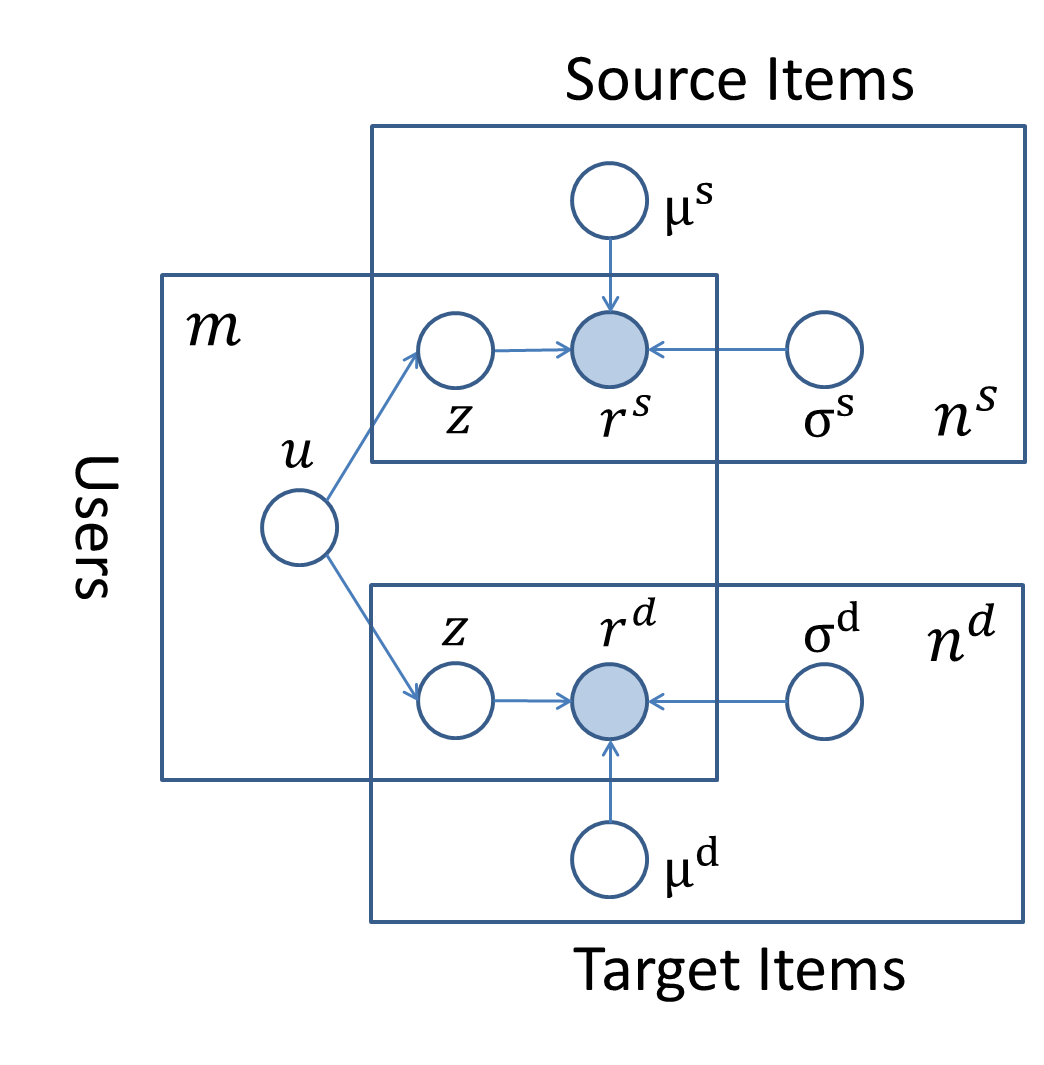
\includegraphics[width=4in]{fig/GM-TGPLSA}
\caption{The graphical model for TGPLSA with one source domain and one target domain.}\label{fig:gmodel1}
\end{figure}

TGPLSA jointly learn the two models for both the source domain and the target domain using a relative weight parameter\footnote{$\lambda \in (0,1)$, which is introduced to represent the tradeoff of source and target information.} $\lambda$. Since the item sets $\Is^s$ and $\Is^d$ are different or even disjoint with each other, there could be inconsistency across domains as we discussed in Section \ref{chp:intro}. Clearly, the more consistent source and target domains are, the more help target task could get from source domain(s). We propose a weighted TLCF model (wTGPLSA) to further analyze this inconsistency in our work by learning item weight vectors $\W^{s} = \{w_i^s\}_{i=1}^{n^s}$ and $\W^{d} = \{w_i^d\}_{i=1}^{n^d}$ of the instances in source and target domain respectively. Then, the objective function in Eq.(\ref{eq:likelihood}) can be extended as:
\begin{eqnarray}\label{eq:tplsa_likelihood}
\Loss = - \sum_{r \in R} ( \lambda \sum_{x_{ui}^s \in \X^s} \log ( w_i^s \cdot Pr(x_{ui}^s = r \mid u^s,i^s ; \theta^s) )  \\\nonumber
+ (1-\lambda) \sum_{x_{ui}^d \in \X^d} \log ( w_i^d  \cdot Pr(x_{ui}^d = r \mid u^d,i^d ; \theta^{d}) ) )
\end{eqnarray}

In our setting, either $u^s = u^d$ or $i^s = i^d$. Besides, since we do not make any assumptions on the range of ratings in either source or target domains, the source domains and target domain may have different rating scales, as we show in the experiment in Section \ref{sec:multSource}.

We adopt the expectation-maximization (EM) algorithm, a standard method for statistical inference, to find the maximum log-likelihood estimates of Eq. (\ref{eq:tplsa_likelihood}).
For the convenience of presentation, in the following derivation, we denote $x_{ui}^l\!=\!r, u^l, i^l$ as $x_{ui}^l$.

In the E-step, we compute the posterior probabilities of the hidden variables, as follows:
\begin{eqnarray}\label{eq:p_z_r}
\nonumber
Pr(z \mid x_{ui}^s) \!=\! \frac{Pr(x_{ui}^s \mid z) Pr(z \mid u^s)}{\sum_{z^{'}} Pr(x_{ui}^s \mid z^{'}) Pr(z^{'} \mid u^s)}\\
Pr(z \mid x_{ui}^d) \!=\! \frac{Pr(x_{ui}^d \mid z) Pr(z \mid u^d)}{\sum_{z^{'}} Pr(x_{ui}^d \mid z^{'}) Pr(z^{'} \mid u^d)}
\end{eqnarray}

Following the similar idea of TPLSA~\cite{DBLP:conf/sigir/XueDYY08}, we assume that a particular user's preferences on the latent topics are the same across different domains. Also notice that $Pr(z \mid u^d)$ and $Pr(z \mid u^s)$ reflect the users' preferences on the latent topics. Thus, we set $Pr(z \mid u^d)$ to be the same as $Pr(z \mid u^s)$ to build an information bridge for knowledge transfer across different systems.

In the M-step, we solve the maximization problem via the following equation:
\begin{eqnarray}\label{eq:p_z_u}
Pr(z|u)\!=\!\frac{\sum_{l \in \{s,d\}}\!\!\lambda_l\! \!\sum_{r \in R}\!\!\sum_{x_{ui}^l \in \X^l_{u*}}\!\!w^l_i Pr(z | x_{ui}^l)  }{\sum_{z^{'}} (\sum _{l \in \{s,d\}}\!\!\lambda_l\!\!\sum_{r \in R}\!\!\sum_{x_{ui}^l \in \X^l_{u*}}\!\! w^l_i Pr(z^{'} | x_{ui}^l) ) }
\end{eqnarray}
And we obtain the following equations for the parameters of the Gaussian distribution:
\begin{eqnarray}\label{eq:p_mu}
\mu_{iz}^l \!=\! \frac{\sum_r\sum_{x_{ui}^l \in \X^l_{*i}} r \cdot Pr(z \mid x_{ui}^l)}{\sum_r\sum_{x_{ui}^l \in \X^l_{*i}} Pr(z \mid x_{ui}^l)}
\end{eqnarray}
\begin{eqnarray}\label{eq:p_sigma}
(\sigma_{iz}^{l})^2 \!=\! \frac{\sum_r\sum_{x_{ui}^l \in \X^l_{*i}} (r-\mu_{iz})^2 Pr(z \mid x_{ui}^l)}{\sum_r\sum_{x_{ui}^l \in \X^l_{*i}} Pr(z \mid x_{ui}^l)}
\end{eqnarray}
After proceeding the EM algorithm by alternating E-step using Eq. (\ref{eq:p_z_r}) with M-step using Eq. (\ref{eq:p_z_u}), (\ref{eq:p_mu}) and (\ref{eq:p_sigma}), finally we compute the expected result in the target domain as
\begin{eqnarray}\label{eq:pred}
\hat x_{ui}^d\!=\!E[r \mid u,i] \!=\! \int_R r Pr(r \mid u, i) dr \!\approx\! \sum_{z} Pr(z \mid u) \mu_{i,z}^d
\end{eqnarray}

\hspace{0.1in}
\section{Parallelization of the models}
Due to the computational complexity as the readers may notice in previous sections, those latent feature models are hard to scale up on very large data sets. As we will discussed in Section \ref{chp:STLCF}, we would like to use the probabilistic latent feature models as base model. Therefore, we will need them to be applied to the real world datasets and converged fast. Thanks to the recent raised parallel computation techniques, such as Hadoop ~\cite{white2012hadoop} and MPI ~\cite{gropp1999using}, we could speed up the models mentioned in previous sections on some relatively large data sets.

\hspace{0.05in}
\subsection{Parallelization of TGPLSA}
\begin{figure}
\centering
\includegraphics[width=5in]{fig/parallelplsa.eps}
\caption{A demonstration of how the matrices are accessed during the computations of the GPLSA model}
\label{fig:parallelplsa}
\end{figure}

We present the logic behind the parallelization of TGPLSA. For the convenience of presentation, we show only the logic in a single domain. It is easy to extend it to multiple domains. As we can see in Figure ~\ref{fig:parallelplsa}, for a given user, only the values from a corresponding column in the user latent matrix and the value from the rating matrix are retrieved to calculate Equation ~\ref{eq:p_z_r} in the E-step. No other values are involved. Similar for the calculations in the M-step. The algorithm is therefore able to be plugged into the Map-Reduce framework.

We implement the parallel program under the MPI framework.

In the following chapters, we demonstrate how to adopt the boosting based framework and apply it to TGPLSA to achieve {\em selective} knowledge transfer from multiple source domains. Notice that other than TGPLSA, our proposed framework can be applied to other generative models to solve various problems.


